\chapter{Puissances et\\grandeurs}\label{ChPuissances}

\vspace{5cm}
\begin{acquis}
\begin{itemize}
\item Savoir calculer la puissance d'un nombre entier relatif.
\item Savoir utiliser les formules de calcul avec les puissances.
\item Savoir calculer avec les puissances de 10.
\item Savoir résoudre des problème en utilisant les puissances.
\end{itemize}
\end{acquis}


\activites  
\begin{activite}[Le triangle de Sierpinski]

\begin{partie}[Répondre avec des 3 et des $\times$ uniquement !]

\begin{minipage}{.62\linewidth}
La figure de départ est un triangle équilatéral violet. On construit à l'intérieur de celui-ci un triangle bleu obtenu en joignant les milieux des côtés du triangle de départ.
\end{minipage}\hfill%
\begin{minipage}{.35\linewidth}
\centering

\includegraphics[width=.8\linewidth]{Pacti1}
\end{minipage}

\vspace{1em}

\begin{minipage}{.35\linewidth}
\centering

\includegraphics[width=.6\linewidth]{Pacti2}
\end{minipage}\hfill%
\begin{minipage}{.62\linewidth}
\begin{enumerate}
\item De la même façon, on construit un petit triangle bleu dans chacun des triangles violets de la figure 1. Combien obtient-on de triangles violets dans la figure 2 ?
\item Imaginons que l'on continue à construire des triangles bleus dans les triangles violets. Combien a-t-on de triangles violets dans la figure 4 ? Puis dans la figure 7 (en n'utilisant encore que des 3 et des signes $\times$) ? Et dans la figure 20 ?
\end{enumerate}
\end{minipage}
\end{partie}

\vspace{1em}

\begin{partie}[Une nouvelle notation : la notation « puissance »]

La notation « puissance » est utilisée pour remplacer des produits comme dans les exemples suivants :
    \begin{itemize}
        \item $9 = \underbrace{3 \times 3}_{\text{2 facteurs}} = 3^2$ qui se lit « 3 au carré » ou « 3 puissance 2 » ou « 3 exposant 2 »,
        
        \item $81 = \underbrace{3 \times 3 \times 3 \times 3}_{\text{4 facteurs}}= 3^4$ qui se lit « 3 puissance 4 » ou « 3 exposant 4 ».
        
        
    \end{itemize}
     
\begin{enumerate}
\item Écris, à l'aide de la notation « puissance », le nombre de triangles violets qu'il y a dans la figure 7 puis calcule ce nombre. Recommence pour la figure 20.
\item À l'aide de ta calculatrice, indique combien il y a de triangles violets dans la figure 13, la figure 18, la figure 10 et enfin dans la figure 15. Existe-t-il un moyen d'effectuer ces calculs facilement avec ta calculatrice ?
\end{enumerate}
\end{partie}
 \end{activite}
 
 
\begin{activite}[Des produits avec 2, 3 et 5]

\begin{partie}\label{PactiP1} Nous allons exprimer certains nombres sous la forme de produits. Dans cette activité, les seuls facteurs autorisés sont : 2 ; 3 et 5. Nous utiliserons la notation « puissance » dès que cela est possible.
Exemples :
        \begin{itemize}
        \item $25 = 5 \times 5$ peut s'écrire $25 = 5^2$ ;
		\item $48 = 2 \times 2 \times 2 \times 2 \times 3$ peut s'écrire $48 = 2^4 \times 3$ ;
		\item $90 = 2 \times 3 \times 3 \times 5$ peut s'écrire $90 = 2 \times 3^2 \times 5$.
		\end{itemize}
\begin{enumerate}
\item\label{Pacti1} Exprime de la même façon les nombres 4 ; 12 ; 27 ; 30 ; 45 et 108. Peut-on exprimer le nombre 26 de la même façon ? Justifie.
\item Un élève a écrit l'égalité suivante : $54 = 2^1 \times 3^3$. En considérant que sa réponse est bonne, combien vaut $2^1$ ?
\item Un élève a écrit l'égalité suivante : $50 = 2^1 \times 3^0 \times 5^2$. En considérant que sa réponse est bonne, combien vaut $3^0$ ?
\item Réécris les trois exemples du départ puis les nombres de la question \ref{Pacti1} sous la forme  $2^a \times 3^b \times 5^c$ ($a$, $b$ et $c$ sont des nombres entiers, éventuellement égaux à 0 ou 1).
\item\label{Pacti2} Trouve le plus possible de nombres inférieurs à 100 qui peuvent s'exprimer sous la forme d'un produit ne comportant que des 2, des 3 et des 5.
\end{enumerate}
\end{partie}


\begin{partie}On peut programmer un tableur pour qu'il calcule un produit lorsqu'on lui indique combien celui-ci comporte de 2, de 3 et de 5.

\begin{minipage}{.62\linewidth}
\begin{enumerate}
\item À l'aide du tableur, vérifie les résultats que tu as obtenus à la partie \ref{PactiP1} question \ref{Pacti2} puis poursuis ta recherche.
\item Comment être certain d'avoir terminé cette recherche ?
\end{enumerate}
\end{minipage}\hfill%
\begin{minipage}{.35\linewidth}
\centering
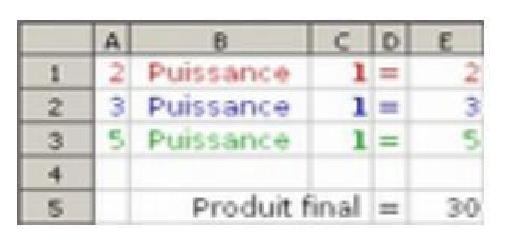
\includegraphics[width=.8\linewidth]{Pacti3}
\end{minipage}
\end{partie}
 \end{activite}
 
 
\begin{activite}[Écriture décimale d'une puissance de 10]
\begin{enumerate}
\item Donne l'écriture décimale des nombres suivants : $10^3$ ; $10^5$ et $10^9$.
\item Recopie puis complète : « L'écriture décimale de $10^{12}$ est un 1 suivi de ... zéros. »
\item Écris sous la forme d'une puissance de 10 les nombres suivants : 
	100 ; 1 000 000 et 1 000 000 000 000 000 000 000.
\item Donne l'écriture décimale des nombres suivants : $10^{-2}$ ; $10^{-6}$ et $10^{-8}$.
\item Recopie puis complète : « L'écriture décimale de $10^{-12}$ comporte ... zéros suivis d'un 1 (la virgule étant placée après le premier ...). »
\item À l'aide de la calculatrice, écris sous la forme d'une puissance de 10 les nombres suivants : 
 0,001 ; 0,000 000 01 et 0,000 000 000 000 000 1.
\end{enumerate}
\end{activite}


\begin{activite}[Toutes sortes de puissances]
\begin{partie}[Des chinois sous différentes formes]

La Chine compte actuellement environ 1 300 000 000 habitants. Donne le nombre d'habitants de la Chine en milliards. Combien cela fait-il en millions ? Et en milliers ?

Complète : $1 300 000 000 = ... \times 10^9 = ... \times 10^6 = ... \times 10^3$.
\end{partie}

\vspace{1em}
\begin{partie}[Distances astronomiques]

Dans le domaine de l'astronomie, le parsec sert à mesurer de très grandes distances entre les astres. Un parsec correspond à environ $3,086 \times 10^{16}$ m.

Complète : 1 parsec = $,086 \times 10^{16}$ m = ... cm = ... km = ... mm.
\end{partie}

\vspace{1em}
\begin{partie}[Globules rouges]

La taille moyenne d'un globule rouge est $7 \times 10^{-6}$ m.

Complète : $7 \times 10^{-6}$ m = ... cm = ... mm.
\end{partie}
\end{activite}

\begin{activite}[Opérations avec des puissances de 10]

\begin{partie}[Produit de puissances de 10]

\[ 10^2 \times 10^3 = \underbrace{\underbrace{10 \times 10}_{\text{... facteurs}} \times \underbrace{10 \times 10 \times 10}_{\text{... facteurs}}}_{\text{... facteurs au total}} = 10^{...}  \qquad \quad 10^5 \times 10^4 = \underbrace{\underbrace{10 \times ... \times 10}_{\text{... facteurs}} \times \underbrace{10 \times ... \times 10}_{\text{...facteurs}}}_{\text{... facteurs au total}} = 10^{...}  \]
      
\begin{enumerate}
\item Recopie puis complète les expressions ci-dessus.
\item Calcule de la même façon : $10^5 \times 10^8$ et $10^7 \times 10^6$.
\item Complète alors la formule suivante : 

Pour tous nombres entiers positifs $n$ et $p$ : $10^n \times 10^p = 10^{...}$.

\end{enumerate}
\end{partie}

\begin{partie}[Quotient de puissances de 10]
\begin{enumerate}
\item Si on décompose $\dfrac{10^5}{10^2}$, on obtient $\dfrac{10 \times 10 \times 10 \times 10 \times 10}{10 \times 10}$.

Simplifie cette fraction et donne le résultat sous la forme d'une puissance de 10.
\item Recommence avec les fractions suivantes : $\dfrac{10^7}{10^5}$ et $\dfrac{10^3}{10^2}$.
\item Complète alors la formule suivante :

Pour tous nombres entiers positifs $n$ et $p$ : $\dfrac{10^n}{10^p}=10^{...}$.
\end{enumerate}
\end{partie}

\begin{partie}[Puissance de puissances de 10]

\begin{enumerate}
\item Compte le nombre de facteurs 10 contenus dans l'écriture décomposée de $(10^2)^3$.
\item Recommence avec $(10^3)^5$. Combien aurait-on de facteurs 10 dans $(10^5)^8$ ?
\item Complète alors la formule suivante : 

Pour tous nombres entiers positifs $n$ et $p$ : $(10^n)^p=10^{...}$.
\end{enumerate}
\end{partie}
\end{activite}



\cours
\section{Puissances entières d'un nombre relatif}

\subsection{Notations $a^n$}

\begin{definition}
Pour tout nombre entier $n$ positif non nul, pour tout nombre relatif $a$ :
\[ a^n = \underbrace{a \times a \times ... \times a}_{\text{$n$ facteurs}} \]
$a^n$ (lu « \textbf{a puissance n} ») est appelé \MotDefinition{puissance}{} $n$-ième de $a$ et $n$ est appelé l'\MotDefinition{exposant}{}.
\end{definition}


\begin{remarque}
Par convention : $a^0=1$. De plus, on a : $a^1=a$
\end{remarque}

\begin{exemple}
Donne l'écriture décimale des nombres : $2^4$ et $10^3$.
\correction
$2^4 = 2 \times 2 \times 2 \times 2 = 16$

$10^3 = 10\times10\times10 = 1 000$
\end{exemple}


\begin{exemple}
Écris sous la forme d'une puissance les expressions : $3^2 \times 3^3$ et $\dfrac{2^5}{2^3}$.
\correction
$3^2 \times 3^3  = (3 \times 3) \times (3 \times 3 \times 3) = 35$

$\dfrac{2^5}{2^3}=\dfrac{2\times2\times2\times2\times2}{2\times2\times2}=2^2$
\end{exemple} 





\subsection{Signe d'une puissance}

\begin{exemple*1}
Calculer les puissances suivantes :
\begin{itemize}
    \item $2^3 =$ 
    \item $5^2 =$ 
    \item $(-3)^4 =$ 
    \item $(-3)^3 =$ 
    \item $(-4)^2 =$ 
    \item $(-4)^3 =$ 
\end{itemize}
\end{exemple*1}

À partir des exemples ci-dessus, on peut conjecturer la propriété suivante : 
 Propriété 

\begin{propriete}
Pour tout nombre entier relatif $n$,
\begin{itemize}
    \item Si $a$ est positif alors $a^n$ est positif.
    \item Si $a$ est négatif alors $a^n$ est : \subitem positif lorsque l'exposant $n$ est pair,
			       \subitem et négatif lorsque l'exposant $n$ est impair.
\end{itemize}
\end{propriete}

\begin{exemple*1}
Quel est le signe de $A = (-3)^4$ et de $B = (-2)^5$ ?
\correction
Comme $-3$ est négatif et l'exposant 4 est pair, $A$ est un nombre positif.

Comme $-2$ est négatif et l'exposant 5 est impair, $B$ est un nombre négatif.
\end{exemple*1}
Exemple : 



\subsection{Utiliser les formules sur les puissances}


\begin{aconnaitre}
Pour tout nombre relatif $a$ non nul et pour tous nombres entiers relatifs $m$ et $p$ :
\[ a^m \times a^p = a^{m+p} \qquad ; \qquad \dfrac{a^m}{a^p}=a^{m-p} \qquad \text{et} \qquad (a^m)^p = a^{m\times p} .\]
\end{aconnaitre}

\begin{exemple*1}
Écris les expressions sous la forme $a^n$, où $a$ est un nombre relatif et $n$ un entier relatif.

$A=5^7 \times 5^4$

$B=\dfrac{(-2)^6}{(-2)^5}$

\correction

$A = 5^7 \times 5^4 = 5^{7+4}=5^{11}$

$B=\dfrac{(-2)^6}{(-2)^5}=(-2)^{6-5}=(-2)^1=-2$
\end{exemple*1}


\begin{exemple*1}
Écris le nombre $C=\dfrac{(-2)^4\times 4^5}{8^2}$ sous la forme d'une puissance de 2.

\correction

\begin{tabular}{lcl}
$C=\dfrac{(-2)^4\times 4^5}{8^2}$ & $\longrightarrow$ & On remplace 4 par 22 et 8 par 23. \\
$C=\dfrac{(-2)^4\times 4^5}{8^2}$ & $\longrightarrow$ & On remarque que (- 2)4 = 24. \\
$C=2^{4+10-6}$ & $\longrightarrow$ & On applique les règles sur les puissances. \\
$C=2^8$ & $\longrightarrow$ & On donne l'écriture demandée par l'énoncé.\\
\end{tabular}
\end{exemple*1}



\begin{aconnaitre}
Pour tous nombres relatifs $a$ et $b$ non nuls et pour tout nombre entier relatif $n$ :
\[ (a\times b)^n = a^n \times b^n  \qquad \text{et} \qquad \left(\dfrac{a}{b}\right)^n = \dfrac{a^n}{b^n} \]
\end{aconnaitre}


\begin{exemple*1}
Écris les expressions suivantes sous la forme $a^n$, où $a$ est un nombre relatif non nul et $n$ un entier relatif.

$D=2^3 \times 5^3$

$E=\dfrac{15^5}{5^5}$

$F=(-6)^5 \times \left(\dfrac{1}{3}\right)^5$

\correction

$D=2^3 \times 5^3 = (2\times 5)^3 = 10^3$

$E=\dfrac{15^5}{5^5} = \left(\dfrac{15}{5}\right)^5 = 3^5$

$F=(-6)^5 \times \left(\dfrac{1}{3}\right)^5 = \left(-6\times \dfrac{1}{3}\right)^5 = (-2)^5 = -2^5$

\end{exemple*1}





\section{Puissances de 10}

\subsection{Notations $10^n$}

\begin{definition}
Pour tout nombre entier $n > 0$ : $10^n=\underbrace{10 \times 10 \times ...\times 10}_{n \text{ facteurs}}=1\underbrace{0...0}_{n \text{ zéros}}$ et $10^0=1$. 

\end{definition}

\begin{exemple*1}
Écris les nombres 1 000, 10 000 000 et 100 000 sous la forme d’une puissance de 10.

\correction

$1 000 = 10^3$

$10 000 000 = 10^7$

$100 000 = 10^5$
\end{exemple*1}


\subsection{Multiplication par une puissance de 10}

\begin{aconnaitre}
Soit $n$ un nombre entier positif non nul.

Multiplier un nombre par $10^n$ revient à décaler la virgule de \textbf{$n$ rangs vers la droite} (on complète par des zéros si nécessaire).
\end{aconnaitre}

\begin{exemple*1}
Donne l'écriture décimale des nombres $208,641 \times 10^2$ et $-37,1 \times 10^4$.

\correction

$208,641 \times 10^2 = 20 864,1$ 

$-37,1 \times 10^4 = -371 000$
\end{exemple*1}


\begin{exemple*1}
Par combien faut-il multiplier 7,532 pour obtenir 75 320 ?

\correction

Pour passer de 7,532 à 75 320, on décale la virgule de \textbf{4 rangs vers la droit}e donc il faut multiplier 7,532 par $10^4$  pour obtenir 75 320.
\end{exemple*1}




\subsection{Calcul avec des puissances de 10}



On considère \textbf{deux nombres entiers relatifs $m$ et $p$}. Les règles de calcul avec les puissances de 10 sont les mêmes qu'avec les nombres relatifs mais elles sont très souvent utilisées : 

\begin{aconnaitre}[Règle de calcul avec deux puissances de 10]
\[ 10^m \times 10^p = 10^{m + p} \qquad ; \qquad \dfrac{10^m}{10^p}=10^{m-p} \qquad ; \qquad \left(10^m\right)^p = 10^{m\times p} \]
\end{aconnaitre} 
		
\begin{exemple*1}

Donne l'écriture décimale du nombre $A = 10^4 \times 10^3$.

\correction

$A = 10^4 \times 10^3 = 10^{4+3} = 10^7 = 10 000 000$
\end{exemple*1}



\begin{exemple*1}
Écris le nombre $B =\dfrac{10^5}{10^2}$ sous la forme d'une seule puissance de 10.

\correction

\begin{tabular}{lcl}
$B = 10^{5-2}$ & $\longrightarrow$ & On applique la règle du quotient de deux puissances de 10. (Attention aux signes moins !) \\
$B = 10^3$ & $\longrightarrow$ & On donne l'écriture demandée par l'énoncé. \\
\end{tabular}
\end{exemple*1}



\begin{exemple*1}
Écris le nombre $C =\left(10^3\right)^7 \times \left(10^2\right)^3$ sous la forme d'une seule puissance de 10.

\correction

\begin{tabular}{lcl}
$C = 10^{3 \times 7} \times 10^{2 \times 3}$ & $\longrightarrow$ & On applique la règle des puissances de puissance de 10. \\
$C = 10^{21} \times 10^6$ & $\longrightarrow$ & On effectue les multiplications sur les exposants. \\
$C = 10^{21 + 6}$ & $\longrightarrow$ & On applique la règle du produit de deux puissances de 10. \\
$C = 10^{27}$ & $\longrightarrow$ & On donne l'écriture demandée par l'énoncé. \\
\end{tabular}

\end{exemple*1}



\begin{remarque}
Attention : il n'y a pas de règle avec l'addition ou la soustraction !
\end{remarque}



\begin{exemple*1}
Donne l'écriture décimale des nombres $F = 10^3 + 10^2$ et  $G = 10^4 - 10^1$.
\end{exemple*1}

\exercicesbase
\begin{colonne*exercice}
\serie{Puissance d'un nombre}

\begin{exercice}[]
Voici une liste de mots : exposant, puissance, facteurs, produit. Recopie chaque phrase en la complétant par le mot qui convient.

\begin{colenumerate}{1} 
\item $3^7$ se lit « 3 ... 7 ».
\item $5^4$ est le ... de quatre ... tous égaux à 5.
\item 8 est l'... de $6^8$.
\item Le ... de six ... égaux s'écrit sous la forme d'une ... d'... 6.
\end{colenumerate} 
\end{exercice}

\begin{exercice}[D'une écriture à l'autre]

\begin{colenumerate}{1} 
\item Écris en toutes lettres : $3^4$ ; $2^3$ ; $7,1^9$ et $(-4)^2$.
\item Écris en expressions mathématiques :
    \subitem huit puissance neuf 
    \subitem quatre au cube 
    \subitem trois puissance cinq 
    \subitem sept au carré
\end{colenumerate} 
\end{exercice}

\begin{exercice}[]\label{Pex1}
Recopie et complète chaque expression par l'exposant manquant :

\begin{colenumerate}{1} 
\item $4 \times 4 \times 4 \times 4 \times 4 \times 4 \times 4 \times 4 \times 4 = 4^{...}$
\item $(-5) \times (-5) \times (-5) \times (-5) \times (-5) = (-5)^{...}$
\item $0,1 \times 0,1 \times 0,1 = 0,1^{...}$
\end{colenumerate} 
\end{exercice}

\begin{exercice}[]
Décompose chaque nombre comme dans l'exercice \RefExercice{Pex1} :

\begin{colenumerate}{3} 
\item $9^4$
\item $2^3$
\item $5^7$
\item $(-7)^5$
\item $5,3^4$
\item $(-0,8)^3$ 
\end{colenumerate} 
\end{exercice}



\begin{exercice}[]
Quels sont les nombres négatifs :

\begin{colenumerate}{3} 
\item $(-6)^4$
\item $6^8$
\item $-132^{51}$
\item $(-12)^{15}$
\item $(-3)^7$
\item $(-3,6)^{100}$
\item $-(-35)^7$
\item $-87^4$
\item $-(-13^8)$
\end{colenumerate} 
 
\end{exercice}


\begin{exercice}[Puissance de 1 ou de $-1$]

Calcule :

\begin{colenumerate}{4} 
\item $1^{12}$
\item $1^0$
\item $(-1)^8$
\item $(-1)^0$
\item $-1^7$
\item $-1^6$
\item $(-1)^9$
\item $-1^0$
\end{colenumerate} 
 
\end{exercice}

\begin{exercice}[Exposant 0 ou 1]

Calcule :

\begin{colenumerate}{4} 
\item $4^0$
\item $0,5^1$
\item $(-6)^0$
\item $1,2^1$
\item $0,5^1$
\item $-5^1$
\item $(-1,8)^1$
\item $-7^0$
\end{colenumerate} 
 
\end{exercice}

\begin{exercice}[]
Décompose puis donne l'écriture décimale en calculant à la main :

\begin{colenumerate}{4} 
\item $2^4$
\item $-2^4$
\item $(-2)^4$
\item $7^2$  
\item $(-3)^4$
\item $-3^4$
\item $(-6)^3$
\end{colenumerate} 
 
\end{exercice}

\begin{exercice}[]
Donne l'écriture décimale en calculant à la calculatrice :

\begin{colenumerate}{4} 
\item $2^{14}$ 
\item $17^{7}$ 
\item $8^{11}$
\item $12^3$
\item $-3^{10}$
\item $(-11)^8$
\item $(-4)^5$
\item $-6^4$
\end{colenumerate} 
 
\end{exercice}

\begin{exercice}[]
Écris les nombres suivants sous la forme d'un produit :

\begin{colenumerate}{1} 
\item de puissances de 2 et de 5 :
    \subitem $A = 2 \times 2 \times 5 \times 5 \times 5 \times 2 \times 2 \times 5 \times 5$
    \subitem $B = 25 \times 10 \times 5 \times 8$
    \subitem $C = 625 \times 512$
\item de puissances de 2, de 3 et de 7 :
    \subitem $D = 2 \times 2 \times 2 \times 3 \times 7 \times 7$ 
    \subitem $E = 32 \times 21 \times 12$ 
    \subitem $F = 12 \times 21 \times 49$
    \subitem $G = 42$
\end{colenumerate} 
\end{exercice}

\begin{exercice}[]
Écris sous la forme d'un produit :

\begin{colenumerate}{1} 
\item de puissances de 2 et de 5 :
    \subitem $A =\dfrac{2\times 2\times 2\times 5 \times 5}{2\times 2 \times 5}$ 
    \subitem $B =\dfrac{25}{4} \times \dfrac{64}{8}$ 
\item de puissances de 2, de 3 et de 7 :
    \subitem $C =\dfrac{2\times 3\times 3\times 7 \times 7}{2\times 3 \times 7 \times 7}$ 
    \subitem $D =\dfrac{2^6\times 3^4\times 7^2}{49\times 32 \times 27}$ 
\end{colenumerate} 
\end{exercice}

\begin{exercice}[]
Écris sous la forme $a^n$, où $a$ est un nombre relatif et $n$ est un entier naturel.

\begin{colenumerate}{2} 
\item $5^2 \times 5^4$
\item $6^5\times 6^8$
\item $3^4 \times 5^4$
\item $-4\times (-4)^7$ 
\item $7^{-5}\times 7$
\item $-2^3\times (-2)^5$
\item $\left(\dfrac{2}{3}\right)^3 \times \left(\dfrac{2}{3}\right)^5$
\end{colenumerate} 
\end{exercice}

\begin{exercice}[]
Écris sous la forme $a^n$, où $a$ est un nombre relatif et $n$ est un entier relatif.
\begin{colenumerate}{3} 
\item $\dfrac{3^8}{3^4}$
\item $\dfrac{6^5}{3^5}$
\item $\dfrac{20^6}{4^6}$
\end{colenumerate} 
 
\end{exercice}

\begin{exercice}[]
Écris sous la forme $a^n$, où $a$ est un nombre relatif et $n$ est un entier naturel.

\begin{colenumerate}{3} 
\item $\left(2^4\right)^3$ 
\item $\left(\left(-5\right)^3\right)^2$
\item $\left(-4^7\right)^8$
\end{colenumerate} 
\end{exercice}

\begin{exercice}[]
Écris sous la forme d'une seule puissance.
\begin{colenumerate}{2} 
\item $A=8^2 \times 8^3 \times 8^7$
\item $B=11^8 \times \dfrac{11^7}{11^4}$
\item $C=\dfrac{\left(-3\right)^6 \times \left(-3\right)^8}{\left(-3\right)^7}$
\end{colenumerate} 
\end{exercice}

\begin{exercice}[]
Recopie et complète.

\begin{colenumerate}{2} 
\item $3^4 \times 3.... = 3^9$
\item $\dfrac{2^6}{2^{...}}=2^5$
\item $4^{...} \times 4^3 = 4^3$
\item $\left(5^{...}\right)^6 = 5^{18}$
\item $\left(\left(-3\right)^2\right)^{...}=\left(-3\right)^{13}$
\end{colenumerate} 
\end{exercice}


\serie{Calculs avec des puissances}




\begin{exercice}[]
Calcule, sans calculatrice, les expressions suivantes :
$A = 3 \times 2^4 + 5 \times 4^3$
$B = 1 + 10 + 10^2 + 10^3 + 10^4 + 10^5$
$C = 1 -3^2 \times (-5)^2$
$D = 2^3 \times (-9) + 3^3 -(5^2 + 2^1)$
\end{exercice}

\begin{exercice}[]

Calcule les expressions suivantes en utilisant ta calculatrice :

\begin{colenumerate}{2} 
\item $25^3-\left(5 + 11\right)^5$
\item $\dfrac{\left(2+7\right)^5}{5-(-2)}$
\item $\left(\dfrac{-3}{8}\right)^4$
\end{colenumerate}
\end{exercice}

\begin{exercice}[]
Écris sous la forme d'une puissance :

\begin{colenumerate}{3} 
\item $3^4 \times 3^2$
\item $4^3 \times 4^{-5}$
\item $(-5)^4 \times (-5)^3$
\item $\dfrac{2^4}{2^5}$
\item $\left(7^2\right)^3$
\item $7^5 \times 2^5$
\item $8^3 \times 4^3$
\end{colenumerate} 
\end{exercice}



\begin{exercice}[]
Calcule astucieusement :
\begin{colenumerate}{2} 
\item $A = 2^4 \times 0,026 \times 5^4$
\item $B = 5^2 \times 2^2 \times 84$
\item $C = 2^3 \times 5^3 \times 2 500$
\item $D = 2^6 \times 36 \times 5^5$
\end{colenumerate}
\end{exercice}



\serie{Puissances de 10}


\begin{exercice}[]
Donne l'écriture décimale des nombres :

\begin{colenumerate}{4} 
\item $10^4$
\item $10^6$ 
\item $10^8$ 
\item $10^0$
\item $10^5$
\item $-10^0$
\item $(-10)^1$
\item $(-10)^{10}$
\end{colenumerate} 
\end{exercice}

\begin{exercice}[]
Écris à l'aide d'une puissance de 10 :

\begin{colenumerate}{1} 
\item 10 000 ; 10 000 000 ; 1 000 000 ; 1 000.
\item cent ; cent mille ; un milliard ; mille milliards.
\end{colenumerate} 
\end{exercice}

\begin{exercice}[Produit de puissances]
Exprime sous la forme d'une puissance de 10 :

\begin{colenumerate}{2} 
\item $10^5 \times 10^7$
\item $10^4 \times 10^{12}$
\item $10^8 \times 10^9$
\item $10^1 \times 10^3 \times 10^2$
\item $10 \times 10^5$
\item $10^6 \times 10^0$
\end{colenumerate} 
\end{exercice}

\begin{exercice}[Quotient de puissances]
Exprime sous la forme d'une puissance de 10 :

\begin{colenumerate}{2} 
\item $\dfrac{10^5}{10^4}$
\item $\dfrac{10^7}{10^2}$
\item $\dfrac{10^3}{10}$
\item $\dfrac{10^4}{10^0}$
\end{colenumerate} 
\end{exercice}

\begin{exercice}[Puissance de puissances]
Exprime sous la forme d'une puissance de 10 :

\begin{colenumerate}{3} 
\item $\left(10^3\right)^7$
\item $\left(10^8\right)^2$
\item $\left(10^0\right)^7$
\end{colenumerate} 

\end{exercice}

\begin{exercice}[Méli-mélo]
Écris chaque expression sous la forme d'une puissance de 10 :

\begin{colenumerate}{2} 
\item $\left(10^9\right)^4$
\item $\dfrac{10^9}{10^4}$
\item $10^{12} \times 10^0 \times 10^5$
\item $\dfrac{10^6}{10^6}$
\item $\dfrac{10^{12}\times 10^5}{10^9}$
\item $10^9 \times 10^{12}$
\item $\dfrac{10^0}{10^8}$
\item $\left(10^3\right)^1$
\item $\left(10^{10}\right)^0$
\item $\dfrac{10^{21}}{10^4 \times 10^{17}}$
\end{colenumerate}
\end{exercice}

\begin{exercice}[]
Recopie et complète par l'exposant manquant. Tu indiqueras sur ton cahier l'opération que tu as effectuée pour trouver ce nombre :

\begin{colenumerate}{2} 
\item $10^4 \times 10^{...} = 10^7$
\item $10^{...} \times 10^7 = 10^{13}$
\item $10^8 \times 10^{...} = 10^8$
\item $10^8 \times 10^{...} = 10^9$
\end{colenumerate} 

\end{exercice}

\begin{exercice}[]
Complète les phrases suivantes :

\begin{colenumerate}{1} 
\item Lorsque je multiplie un nombre positif par $10^3$, j'obtiens un résultat ... fois plus ... que le nombre de départ.
\item Lorsque je divise un nombre positif par $10^2$, j'obtiens un résultat ... fois plus ... que le nombre de départ.
\end{colenumerate}
\end{exercice}

\end{colonne*exercice}


%\exercicesappr
%\begin{colonne*exercice}
%\input{Puissances/Puissances_exos_approf}
%\end{colonne*exercice}

\connaissances
\QCMautoevaluation{Pour chaque question, plusieurs réponses sont proposées. Déterminer celles qui sont correctes.}

\begin{QCM}
\begin{GroupeQCM}

\begin{exercice}
$5^3=...$
\begin{ChoixQCM}{4}
\item $15$
\item $8$
\item $125$
\item $\dfrac{1}{125}$
\end{ChoixQCM}
\begin{corrige}
\reponseQCM{a}
\end{corrige}
\end{exercice}

\begin{exercice}
$-2^4=...$
\begin{ChoixQCM}{4}
\item $-2 \times 2 \times 2 \times 2$
\item $(-2)4$
\item $-8$
\item $-16$
\end{ChoixQCM}
\begin{corrige}
\reponseQCM{a}
\end{corrige}
\end{exercice}

\begin{exercice}
$\left(-1\right)^{123}=...$
\begin{ChoixQCM}{4}
\item $-123$
\item $-1$
\item $1$
\item $0$
\end{ChoixQCM}
\begin{corrige}
\reponseQCM{a}
\end{corrige}
\end{exercice}

\begin{exercice}
$10^3=...$
\begin{ChoixQCM}{4}
\item mille
\item $10 \times 100$
\item $100$
\item $0,001$
\end{ChoixQCM}
\begin{corrige}
\reponseQCM{a}
\end{corrige}
\end{exercice}

\begin{exercice}
$2\times 3^2$
\begin{ChoixQCM}{4}
\item $6^2$
\item $18$
\item $2\times 9$
\item $36$
\end{ChoixQCM}
\begin{corrige}
\reponseQCM{a}
\end{corrige}
\end{exercice}

\begin{exercice}
$-\left(\dfrac{1}{2}\right)^2=...$
\begin{ChoixQCM}{4}
\item $-\dfrac{2}{4}$
\item $\dfrac{1^2}{2}$
\item $\dfrac{2}{4}$
\item $\dfrac{1}{4}$
\end{ChoixQCM}
\begin{corrige}
\reponseQCM{a}
\end{corrige}
\end{exercice}

\begin{exercice}
Fin 2006, la population mondiale était d'environ 6 500 000 000 habitants. Ce nombre peut s'écrire...
\begin{ChoixQCM}{4}
\item $65 \times 10^8$
\item $6,5 \times 10^9$
\item $650 \times 10^9$
\item $0,65 \times 10^{10}$
\end{ChoixQCM}
\begin{corrige}
\reponseQCM{a}
\end{corrige}
\end{exercice}

\begin{exercice}
$6,4 \times 10^7 = ...$
\begin{ChoixQCM}{4}
\item $6,47$
\item $6,400 000 00$
\item $64 000 000$
\item $0,000 000 64$
\end{ChoixQCM}
\begin{corrige}
\reponseQCM{a}
\end{corrige}
\end{exercice}

\begin{exercice}
Mille milliards de mille sabords est égal, en sabords, à...
\begin{ChoixQCM}{4}
\item $10^3 \times 10^9 \times 10^3$
\item $1^{15}$
\item $10^{81}$
\item $10^{15}$
\end{ChoixQCM}
\begin{corrige}
\reponseQCM{a}
\end{corrige}
\end{exercice}

\begin{exercice}
$10^6 + 10^4 = ...$
\begin{ChoixQCM}{4}
\item $1 010 000$
\item $10^{10}$
\item $10^{24}$
\item $1,01\times 10^6$
\end{ChoixQCM}
\begin{corrige}
\reponseQCM{a}
\end{corrige}
\end{exercice}

\begin{exercice}
$4 + 2 \times 5^3 = ...$
\begin{ChoixQCM}{4}
\item $14^3$
\item $1 004$
\item $254$
\item $6 \times 15$
\end{ChoixQCM}
\begin{corrige}
\reponseQCM{a}
\end{corrige}
\end{exercice}

\end{GroupeQCM}
\end{QCM}


%\TravauxPratiques
%\input{Puissances/Puissances_enGrp.tex}

\Recreation % avec R majuscule pour saut de page
\begin{enigme}[Curiosité...]

Montre que la différence $10^3 -6^3$ est un carré (c'est-à-dire qu'elle peut s'écrire $n^2$, $n$ étant un entier) et que la différence $10^2 -6^2$ est un cube (c'est-à-dire qu'elle peut s'écrire $m^3$, $m$ étant un entier).

En fait, 6 et 10 sont les deux plus petits nombres qui sont tels que la différence de leurs cubes est un carré et la différence de leurs carrés, un cube !
\end{enigme}

\vspace{2em}

\begin{enigme}[Calcul impossible ?]
6 103 515 625 est une puissance de 5 et 16 777 216, une puissance de 2 : avec ta calculatrice, trouve lesquelles !

Calcule $6 103 515 625 \times 16 777 216$ sans utiliser la calculatrice cette fois !!
\end{enigme}

\vspace{2em}

\begin{enigme}[Je cherche !]
Quel est le chiffre des unités de $13^1$ ?

Celui de $13^2$ ? De $13^3$ ? De $13^4$ ? De $13^5$ ?
Quel est le chiffre des unités de $13^{2000}$ ?
\end{enigme}


